\section{Results}


\subsection{Number of iterations}

\begin{figure}[htp]
  \centering
  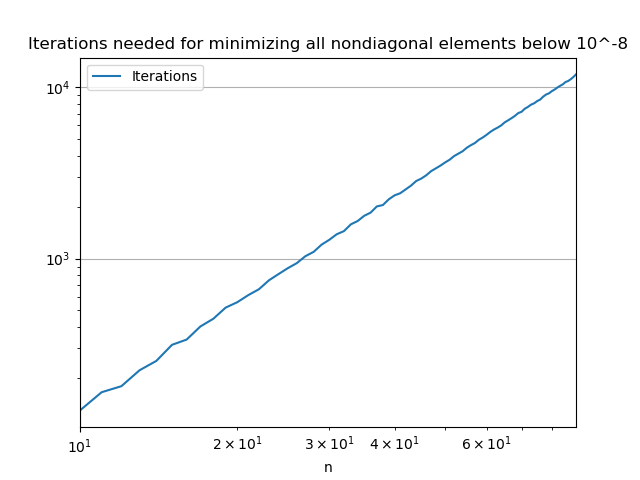
\includegraphics[width=0.66\textwidth]{../figures/iterations.png}

  \caption{Runs of the Jacobi method implemented in c++. Number of iterations
  needed to make all offdiagonal elements smaller than 10$^{-8}$ as function of
  matrix size n.}

  \label{fig:iterations}
\end{figure}


\subsection{Jacobi method c++ run time vs armadillo}

\begin{figure}[htp]
  \centering
  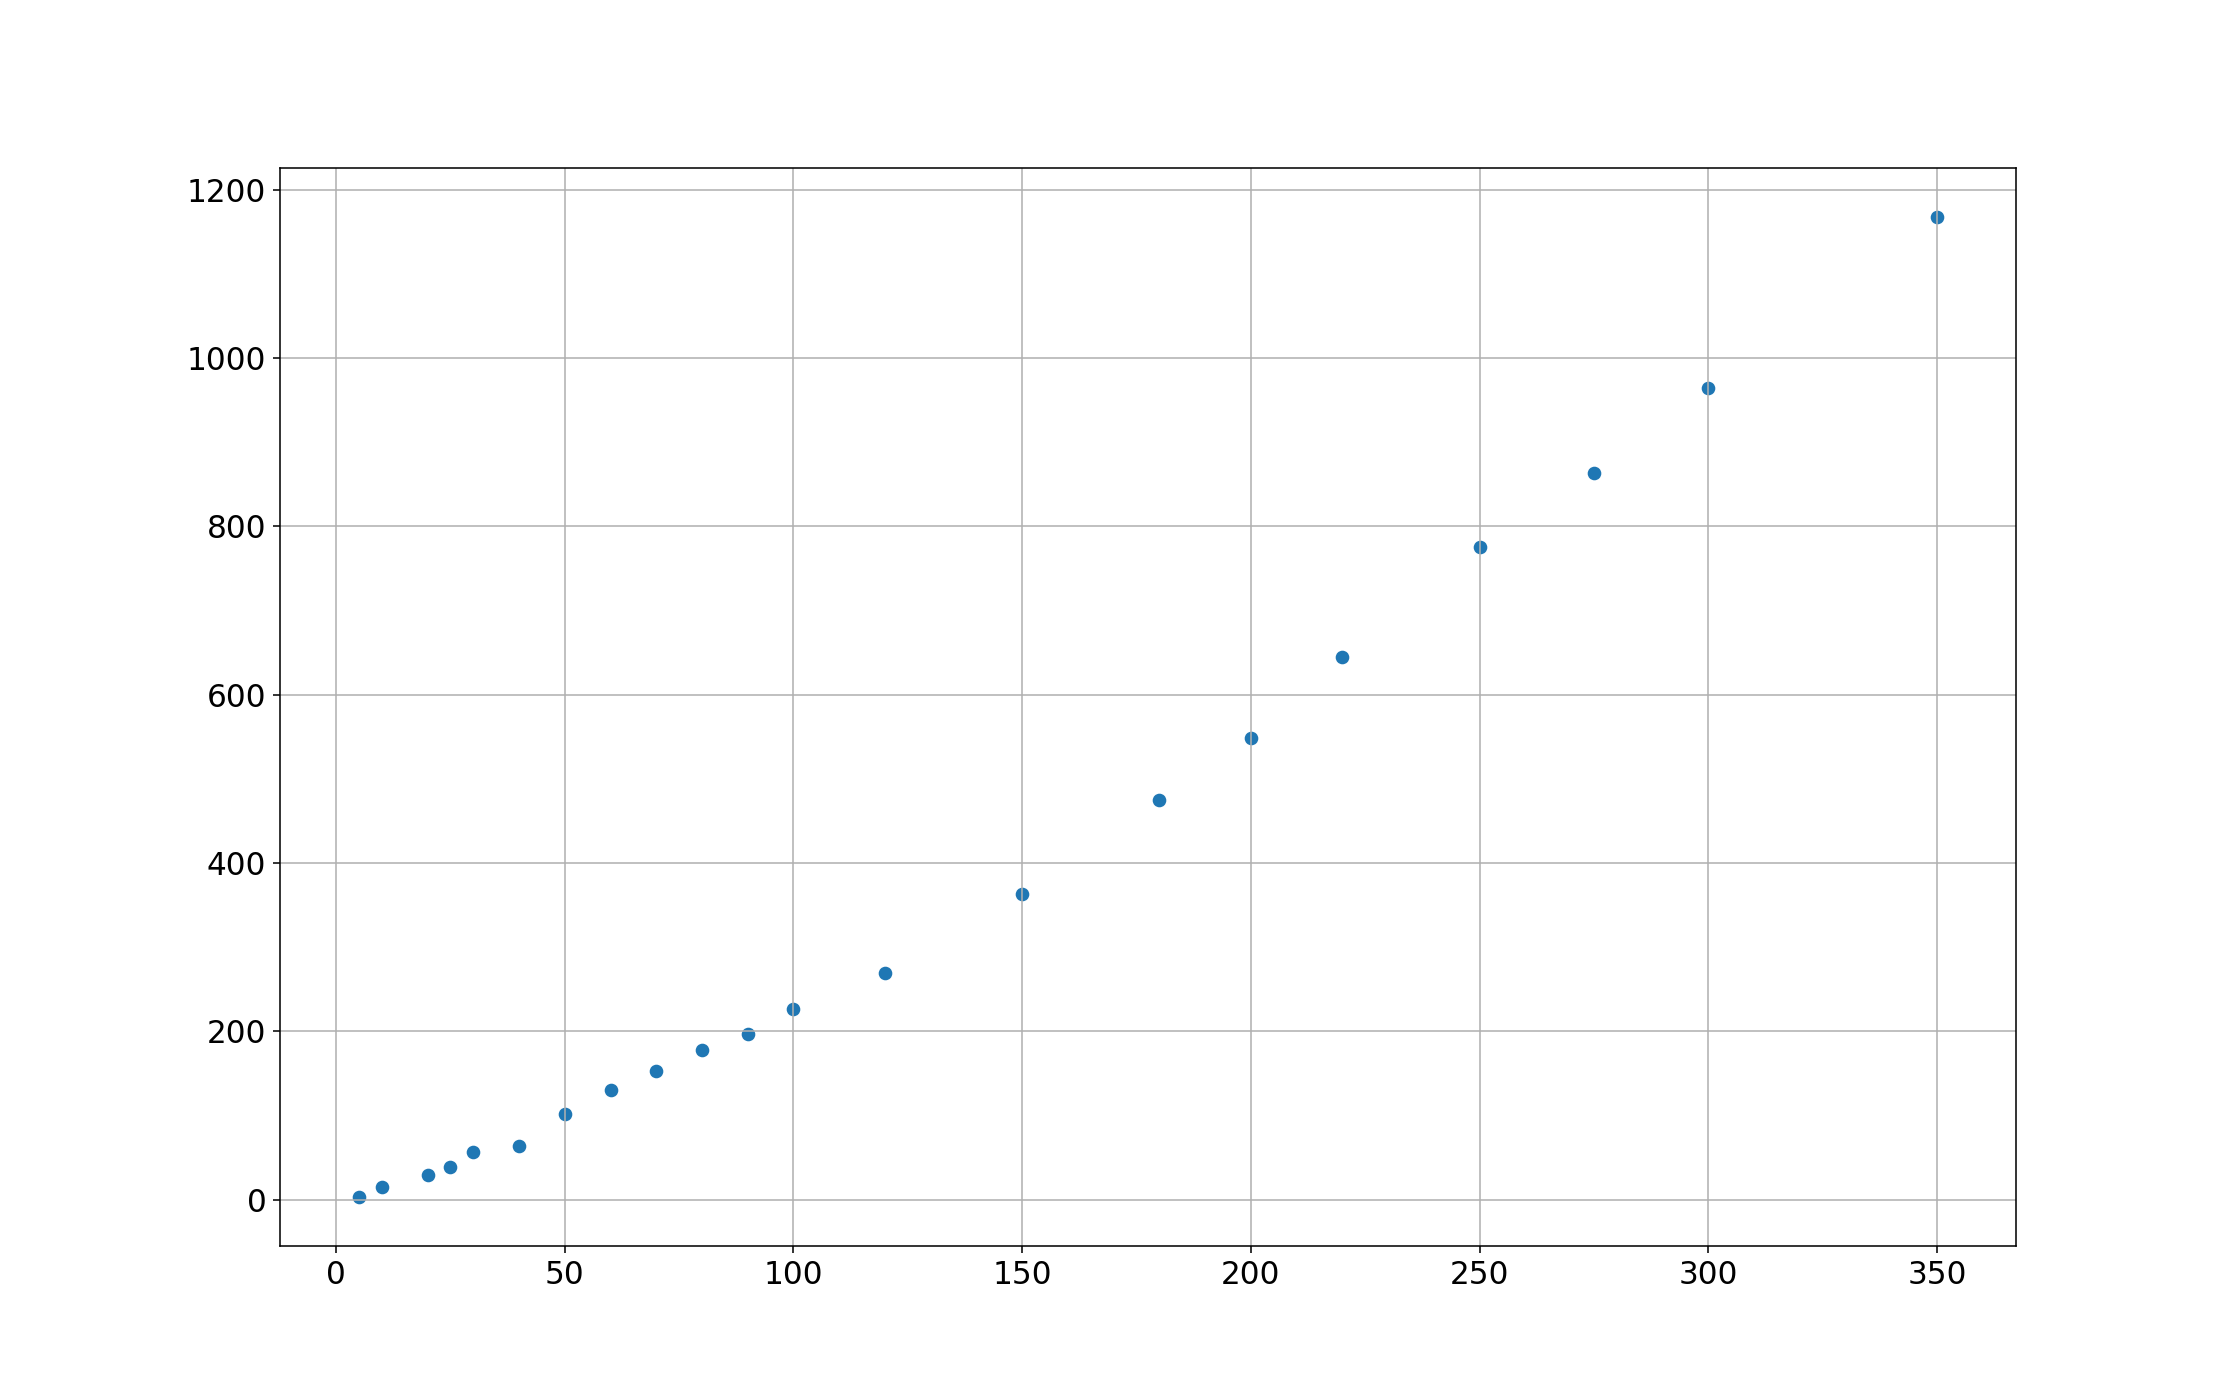
\includegraphics[width=0.66\textwidth]{../figures/compare_arma_cpp.png}

  \caption{Run time of the Jacobi method implemented in c++ divided by the run time of eigsys
  from armadillo. Average of three runs for all n.}

  \label{fig:cpp_arma}
\end{figure}




\subsection{Comparing run times of different implementations of the Jacobi method}
